\chapter{Modelling Autofluorescence in Skin for Novel Biomarkers of Cardiovascular Diseases}
\label{chap:salvo}

% explain it is hard to determine which fluros contribute to signal, and where from within skin can try to sue mcrt to alleviate this

% motivation
% explain fluro method
% explain skin model
% explain nelder mead
% explain filter choice

% results in "2d" 
% results in 3d + higher
% future work

\section{Introduction}


\Gls*{cvds} are the leading cause of death in the world~\cite{whodeath}.
It is estimated that around 18 million people died in 2016 from \gls*{cvds}, accounting for 31\% of global deaths~\cite{whodeath}.
Despite decreasing burden of \gls*{cvds} in the UK, it was still the number two cause of death in the UK in 2014~\cite{bhatnagar2016trends}.

Currently risk factors are used to try to determine if a patient has \gls*{cvd}.
However, these risk factors are only a ``causal pathway leading to the disease''~\cite{vasan2006biomarkers}.

The risk factors such as high blood pressure, smoking, diabetes, physical inactivity, and dyslipidemia do not fully explain incidence of disease~\cite{olsen2010assessment,folsom2013classical}.
Therefore research has moved to examining more novel biomarkers for detecting the disease.
Among these novel biomarkers, the autofluorescence response of tissue is of much interest.

Autofluorescence is the natural fluorescence released by biological structures upon excitation by light.
Autofluorescence is particularly attractive as a biomarker as it requires no exogenous dyes, which can be toxic, non-specific, or interfere with biological function~\cite{kollias1998endogenous}.
In tissue there are several fluorophores responsible for this autofluorescencent response, including: NADH (nicotinamide adenine dinucleotide), structural proteins like collagen and elastin, aromatic amino acids (tyrosine and tryptophan), porphyrins, and FAD (flavin adenine nucleotide)~\cite{monici2005cell}.
Changes in the autofluorescencent response of tissue has been linked to cancer, Alzheimers, diabetes and \gls*{cvds}~\cite{drakaki2009laser,pu2013native,ramanujam2000fluorescence,tarnawska2018pilot,van2019skin}.
Autofluorescence can be linked to these diseases as the fluorophores responsible for the autofluorescence either originate in the mitochondria, or are involved in important biochemical pathways that regulate apoptosis, free-radical generation, oxidative stress and bimolecular sensing of glucose, oxygen and nitric oxide.

NADH has recently been the subject of interest in particular as a biomarker for \gls*{cvds}~\cite{akbar2014vivo,elahi2009oxidative,blacker2016investigating}.
NADH is a intracellular co-enzyme that is a biomarker for metabolic activity and mitochondrial anomalies. 
NADH is involved in mitochondrial function, energy metabolism, calcium homoeostasis, gene expression, oxidative stress, ageing, apoptosis and glycolysis (see~\cref{fig:nadhfadpath}).
Therefore if there is dysfunction, then the autofluroecnet signal from NADH will be affected, thus it can be used as biomarker for disease.

%explain how nadh for cvds and not anything else

Despite their appeal using these autofluorescence to diagnose and asses disease risk more research needs to be carried out on various unknowns: information on the location of fluorescence, which fluorophores contribute to the signal and how much, how much the optics of tissue affect the signal, and the variability of the signal over different location on the body.
This chapter aims to determine how much the tissue optics affects the autofluorescencent signal, which fluorophores contribute to the signal, and from which layer of the skin do they contribute from.
Finally we introduce our ameboaMCRT algorithm, created to determine the relative concentrations of the intrinsic fluorophores in the skin, to assess clinical outcomes.


\begin{figure}[!htpb]
  \centering
  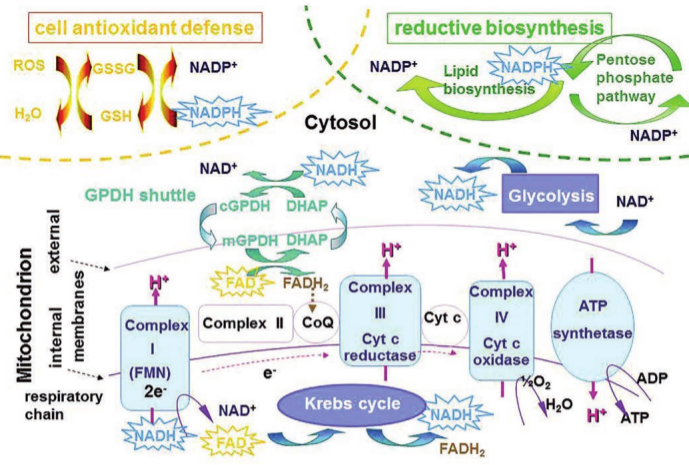
\includegraphics[width=0.75\textwidth]{nadh-cycle.png}
  \caption{Simplified schematic showing the roles of NADH and FAD in various different metabolic pathways. The star boxes indicate fluorescing forms of NADH and FAD. Taken from Croce \textit{et al.}~\cite{croce2014autofluorescence}.}
  \label{fig:nadhfadpath}
\end{figure}


\FloatBarrier

\section{Skin Model}

So far in this thesis all tissue models have been simplified, by assuming that tissue is a homogeneous structure with uniform optical properties.
However, this is not the case in reality.
Tissue is un-homogeneous, with nonuniform optical properties.
However, to create a one to one model of tissue in a simulation is impractical due to the resolution required to resolve all the constituent parts of the tissue down to the cell level.
Therefore we need to make a compromise between reality and what is possible to model efficiently.
This section presents a five layer model of human skin. 

Dermatologists split the skin into several layers based upon the morphology, function and contents of each layer~\cite{freedberg1999fitzpatrick,zaidi2010dermatology}.
The layers named from outer layer to inner most layer: Stratum corenum, Stratum lucidum, Stratum granulosum, Stratum spinosum, Stratum basale, Papillary dermis, Reticular dermis, and Hypodermis.
As not all these layers are optically distinct, are too small to model or not present in a given location on the body.
Therefore, we simplify the layers into just 5 layers: Stratum Corneum, Epidermis, Papillary Dermis, Reticular Dermis, and Hypodermis, with the epidermis compromising of Stratum lucidum, Stratum granulosum, Stratum spinosum, Stratum basale.\Cref{fig:skinexample} shows the geometry of this model.

\begin{figure}[!htpb]
    \centering
    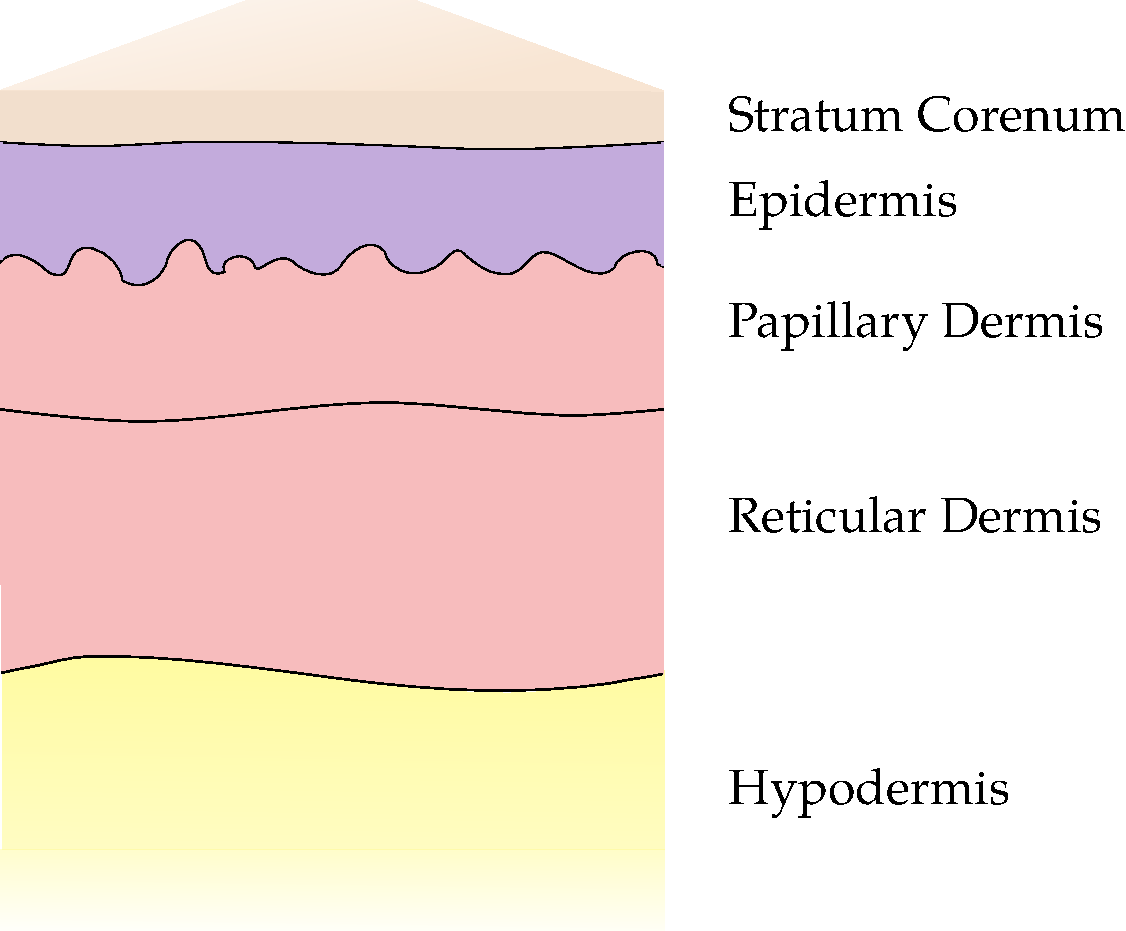
\includegraphics[width=0.7\textwidth]{Skin_layers.pdf}
    \caption{Illustration of our five layer skin model.}
    \label{fig:skinexample}
\end{figure}

Each of these layers have various amounts of chromophores and scatterers.
To accurately model these various chromophores and scatterers, and therefore the skin, we must discuss the biological make up and spatial structure of the skin.

\subsection*{Stratum Corenum} % (fold)
\label{sub:stratum}

The outer most layer of the skin is the Stratum corenum.
This layer mostly consists of dead skin cells (keratinocytes).
Keratinocytes, which make up approximately 80 percent of the cells in the epidermis, are born in the stratum basale, and live for approximately 14 days.
During this period they move upwards to the surface of the skin undergoing a series of complex morphological and metabolic events, which ends with the cells undergoing apoptosis by the time the reach the stratum corenum.
The keratinocytes are flat in shape, cornified and stacked on top each other in this layer.
The function of this layer is to be a protection barrier to prevent damage, infection and diffusion of unwanted chemicals further into the skin.
The stratum corenum also prevents water loss and provides some UV protection~\cite{freedberg1999fitzpatrick,zaidi2010dermatology}.

% subsection stratum_corenum (end)

\subsubsection*{Epidermis} % (fold)
\label{ssub:epidermis}

Below the Stratum corenum is the epidermis.
The epidermis consist of several layers that are optically similar so we restrict our model to modelling this as one whole layer.
The layers that make up the epidermis are the stratum basale, stratum spinosum, stratum granulosum, and the stratum lucidum\footnote{The stratum lucidium only appears in areas of the body where skin is thick, e.g the palm or the sole of the foot.}.
Each of these layers are distinct from one another, in the fact that the keratinocytes in each layer are different from one another.
In the stratum lucidium the keratinocytes are dead, and fairly flat.
The stratum granulosum the keratinocytes are grainy are becoming fairly flat in comparison to the below layers.
Stratum spinosum, the keratinocytes appears spiny (hence the name of the layer), and are polyhedral in shape.
It is in the stratum spinosum that the cells begin to become keratinized and start the process of dying as they move upwards.
Finally the last layer of the epidermis, the startum basale, is the layer where the keratinocytes are born.
Here the keratinocytes are columnar or cuboid in shape.

The purpose of the epidermis is as before to provide a protective barrier to the underlying layers. 
In the stratum basale there is also melanocytes which produce the pigment melanin which is responsible for the color of the skin, and providing some protection from harmful UV light. 
Other types of cells found in the epidermis are Langerhans cells and Merkel cells which are part of the immune system and nervous system respectively.
Overall the epidermis provides protection from mechanical stress, flexibility to the skin, UV protection, retains water, and stops foreign bodies or chemicals from entering the skin~\cite{freedberg1999fitzpatrick,zaidi2010dermatology}.

% subsubsection epidermis (end)

\subsection*{Dermis} % (fold)
\label{sub:dermis}
The dermis is the layer of skin below the epidermis, and makes up the majority of the skin by size.
The cellular makeup of the dermis is different from that of the epidermis, as the dermis is mostly made up of filamentous or fibrous proteins such as elastin or collagen.
The dermis also contains various nerves and blood vessels.
The dermis is split into three layers, the papillary dermis, the reticular dermis, and the hypodermis.
The boundary between the papillary and reticular layers is demarcated by the subpapilliary plexus, which is a horizontal plane of blood vessels.
The boundary between the reticular and the hypodermis is marked by a abrupt change from fibrous to adipose tissue.
The function of the dermis is to protect from mechanical injury, thermal regulation, contains receptors of sensory stimuli, gives the skin pliability, elasticity and tensile strength~\cite{freedberg1999fitzpatrick,zaidi2010dermatology}.
 

% subsection dermis (end)

\subsubsection*{Optical Properties} % (fold)
\label{sub:optical_properties}


%refractive indices from mm02
%blood from louise + inglesias
%melanin from louise + layers thickness
% bilirubin from krishnaswamy04 et al
% carotene  from krishnaswamy04 et al
%water from mm02

With a discussion of what makes up the skin, and what molecules contribute to the skins optical properties, this section gives an account of how our skin model models the optical properties of skin.
First we will discuss the absorber that are found in the skin, and what their absorption properties are as a function of wavelength.
Scattering properties of the several layers of tissue will then be discussed followed by a quick discussion on refractive indices and anisotropy values.
Finally a discussion on the fluorophore found in the skin will be presented.


The first chromophore we will examine is blood.
To model blood, we first split blood into its deoxygenated and oxygenated components.
This is done as the absorption coefficient differs between the two types of blood. We mix these two groups using the tissue oxygenation coefficient $S$. Blood absorption spectra are taken from S. Prahl~\cite{prahlblood}.

\begin{equation}
\mu_{a,Oxy/DeOxy}=150\ \ln10\ \frac{\epsilon}{64458}
\label{eqn:oxy}
\end{equation}

\begin{equation}
\mu_{a,blood}(\lambda) = S\mu_{a,Oxy}+(1-S)\mu_{a,DeOxy}
\label{eqn:blood}
\end{equation}

\noindent Where:

\indent $\epsilon$ is the excitation coefficient of hemoglobin [$cm^{-1}$];

\indent $64458$ is the molecular weight of hemoglobin [$g\ mol^{-1}$];

\indent $150$ is the normal concentration of hemoglobin in blood [$g\ L^{-1}$];

\indent and $\mu_{a,Oxy}$, $\mu_{a,DeOxy}$, and $\mu_{a,blood}$ are the absorption coefficients for oxygenated, deoxygenated and blood respectively [$cm^{-1}$].

\medskip

We also include water in our skin model.
Water's absorption spectrum is taken from the work of Wieliczka \textit{et al} and Segelstein~\cite{wieliczka1989wedge,segelstein1981complex}.

The next chromophores are bilirubin and $\beta$-carotene.
These chromophores are yellow/orange pigments. 
Bilirubin is usually responsible for the yellow skin colour seen in people with jaundice~\cite{jacques1997developing}.
The spectra are taken from S. Prahl's compilation of PhotochemCAD data~\cite{prahlcaro,prahlbili}.

\begin{equation}
\mu_{a,Bilirubin}(\lambda)=\frac{\epsilon_{bilirubin}}{585}\ ln10\ C_{bilirubin}
\label{eqn:bili}
\end{equation}

\begin{equation}
\mu_{a,\beta-Caro}(\lambda)=\frac{\epsilon_{\beta-Caro}}{537}\ ln10\ C_{\beta-Caro}
\label{eqn:caro}
\end{equation}

\noindent Where:

\indent $\epsilon_{bilirubin}$ and $\epsilon_{\beta-Caro}$ are the excitation coefficients for bilirubin and $\beta$-carotene 

\indent respectively [$cm^{-1}$];

\indent $585$, and $537$ are the molecular weights of bilirubin and $\beta$-carotene [$g$];

\indent finally, $C_{bilirubin}$, and $C_{\beta-Caro}$ are the contaminations of bilirubin and $\beta$-carotene 

\indent in the skin [$g\ L^{-1}$].

\medskip

Melanin is the next chromophore we model.
To model melanin's absorption coefficient we use~\cref{eqn:melanin}, taken from~\cite{iglesias2015biophysically}.

\begin{align}
\mu_{a,eumel}(\lambda)&=6.66\times10^{11} \times \lambda^{-3.33}\\
\mu_{a,phomel}(\lambda)&=2.9\times10^{15} \times \lambda^{-4.75}
\label{eqn:melanin}
\end{align}

Finally we use a base absorption coefficient to model the absorption due to the other parts of the skin that contribute to its optical properties, but individually do not have a large effect.
The equation for modelling this was taken from I. Sahdi~\cite{saidi1992transcutaneous}.

\begin{equation}
\mu_{a,base}=7.84\times10^{8}\times\lambda^{-3.255}
\label{eqn:base}
\end{equation}


\Cref{fig:absorcoeff} shows the absorption spectra for the above chromophores as a function of wavelength.

\begin{figure}[!htpb]
	\centering
	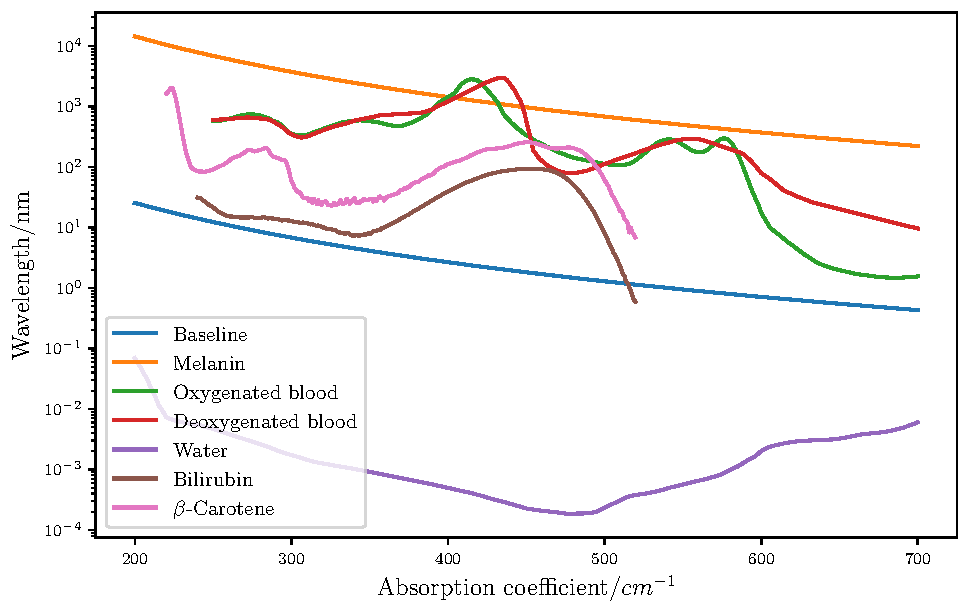
\includegraphics[width=0.75\textwidth]{absorbs.pdf}
	\caption{Absorption coefficients for the various chromophores found in skin.}
	\label{fig:absorcoeff}
\end{figure}

With the absorption properties of the various chromophores in the skin defined we can now discuss the scattering properties of the skin.
As the scattering properties do not vary from layer to layer by too much we use the same equation to describe the scattering coefficient~\cite{jacques2013optical,iglesias2015biophysically,louisethesis}.

\begin{equation}
\mu'_s(\lambda)=a'\left(f_{ray}\left(\frac{\lambda}{500(nm)}\right)^4+(1-f_{ray})\left(\frac{\lambda}{500(nm)}\right)^{-b_{\text{mie}}}\right)
\label{eqn:scattrest}
\end{equation}

\begin{equation}
\mu'_s(\lambda)=1050.60\times\lambda^{-0.68}
\label{eqn:hyposcat}
\end{equation}


\noindent Where:

	$\mu'_s$ is the reduced scattering coefficient [$cm^{-1}$];

	$a'$ is a scaling factor [$cm^-1$];

	$f_{ray}$ is the fraction of Raylieigh scattering [-];

	$\lambda$ is the wavelength of light [$m$];

	and $b_{\text{mie}}$ is the ``scattering power'' [-].

\medskip

This equation mixes both Mie and Rayleigh scattering into one equation.
The first term represents the Rayleigh scattering terms, whilst the second represents the Mie scattering term.
\Cref{fig:scatplot} shows the reduced scattering coefficients for the different layers of the skin.

\begin{table}[!htpb]
  \centering

  \begin{tabular}{|c|c|c|c|}
  \hline

  Layer & $a'/cm^{-1}$ & $f_{ray}$ & $b_{mie}$ \\
  \hline
   Epidermis         & 66.7 & 0.29 & 0.69 \\
   Dermis  & 43.6 & 0.41 & 0.35 \\

  \hline
  \end{tabular}
  \caption{Values of the constants for the scattering equations for the different layers of our skin model. Here epidermis represents the stratum corenum and the epidermis, and dermis represents the papillary, reticular and hypodermis in our model.}
  \label{tab:valscat}

\end{table}

\begin{figure}[!htpb]
	\centering
	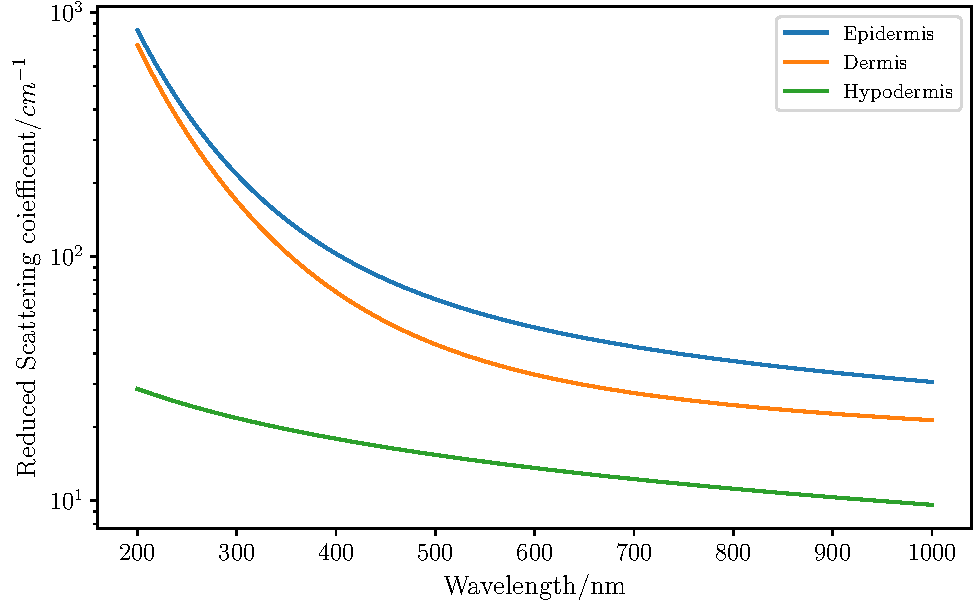
\includegraphics[width=0.75\textwidth]{scat-plot.pdf}
	\caption{Figure shows the reduced scattering coefficient for the different layers of our skin model.}
	\label{fig:scatplot}
\end{figure}



\begin{equation}
\mu_{a,strat}= ((0.1 - 0.3\times10^{-4}\cdot\lambda) + (0.125(\lambda/10.))\times \mu_{a,b}(\lambda))\times(1. - W) + W\cdot\mu_{H_20}(\lambda)
\label{eqn:stratabs}
\end{equation}

\begin{equation}
\begin{split}
\mu_{a,epi}= (\nu_m \cdot (\mu_{phomel}(\lambda) + \mu_{eumel}(\lambda)) + (\mu_{a,b}(\lambda) + \ln10 \cdot \mu_{a,\beta-caro}(\lambda) \cdot C_{caro}) \\ \times (1. - \nu_m)) \times(1. - W) + W \cdot \mu_{H_2O}(\lambda)
\end{split}
\label{eqn:epiabs}
\end{equation}

\begin{equation}
\begin{split}
\mu_{a,pap}=((S \cdot \mu_{a,oxy}(\lambda) + (1. - S) \cdot \mu_{a,deoxy}(\lambda) + \ln10 \cdot \mu_{a,\beta-caro}(\lambda) \cdot C_{caro} + \\ \ln10 \cdot \mu_{a,bili}(\lambda)\cdot C_{bili})\cdot B + \mu_{a,b}(\lambda) \times (1. - B)) \times (1. - W) + W \cdot \mu_{H_2O}(\lambda)
\end{split}
\label{eqn:dermisabs}
\end{equation}

\begin{equation}
\begin{split}
\mu_{a,hypo}=((S\  \mu_{a,oxy}(\lambda) + (1. - S) \times \mu_{a,deoxy}(\lambda)) \times B + \mu_{a,b}(\lambda) \cdot (1. - B))\\ \times (1. - W) + W \cdot \mu_{a,H_2O}(\lambda)
\end{split}
\label{eqn:hypoabs}
\end{equation}


To create our five layer skin model, we mix different amounts of the above chromophores to match what appears in each layer.
\Cref{tab:optpropsvals} shows the amount of each chromophore is included in each layer.


\begin{table}[!tbhp] 
    \begin{adjustwidth}{-.5in}{-.5in}  

  \begin{center}
  \begin{tabular}{|c|c|c|c|c|c|c|c|}
  \hline
  Layer & Thickness/ & Refractive & Blood & Melanin & Bilirubin/ & $\beta$-Carotene/ & Water\\
    &cm & index & volume/\% & volume/\% & $gL^{-1}$ & $gL^{-1}$ & volume/\%\\
  \hline
  Stratum Corenum  & 0.02 & 1.50  & 0.0 & 0.0 & 0.0  & 0.0 & 0.05\\
  Epidermis        & 0.08 & 1.34  & 0.0 & 1.0 & 0.0  & 2.1e-4 & 20.0\\
  Papillary Dermis & 0.18 & 1.40  & 6.0 & 0.0 & 0.05 & 7e-5 & 50.0\\
  Reticular Dermis & 1.82 & 1.395 & 4.5 & 0.0 & 0.05 & 7e-5 & 70.0\\
  Hypodermis       & 5.90 & 1.41  & 5.0 & 0.0 & 0.0  & 0.0 & 70.0\\

  \hline
  \end{tabular}
    \caption{Table of values used for the various concentrations and volumes fraction of the chromophores in the five layer skin model. Values taken from~\cite{krishnaswamy2004biophysically,meglinski2002quantitative,campbell20153d,iglesias2015biophysically}.}
  \label{tab:optpropsvals}
  \end{center}
      \end{adjustwidth}

\end{table}


\begin{figure}[!htpb]
  \centering
  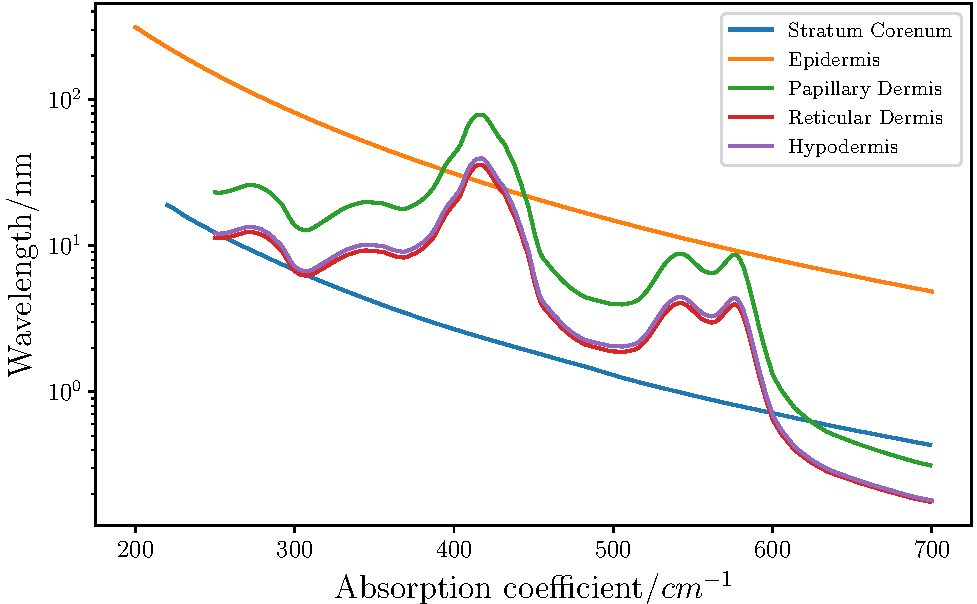
\includegraphics[width=0.75\textwidth]{optical-props.pdf}
  \caption{Absorption coefficients for the different layers in the skin.}
  \label{fig:absoplayers}
\end{figure}

\FloatBarrier

Finally we discuss the anisotropy values and refractive indices of our model.

First, the anisotropy g value is dependant on wavelength~\cite{louisethesis,van1989skin}.

\begin{equation}
g(\lambda)=0.62+0.29\lambda\times10^{-3}
\end{equation}

\noindent Where:

\indent g is the anisotropy value [$-$];

\indent $\lambda$ is the wavelength [$nm$].

The refractive indices of each layer is broadly the same and does not vary form layer to layer by a large amount.
\Cref{tab:refindex} shows the refractive indices adopted for our skin model.

\begin{table}[!htpb]
  \centering

  \begin{tabular}{l|c}
  \hline

  \hline
  Layer & Refractive index \\
  \hline
    Stratum corenum & 1.5 \\
    Epidermis &  1.34\\
    Papilliary dermis & 1.40 \\
    Reticular dermis &  1.395\\
    Hypodermis &  1.41\\

  \hline
  \end{tabular}
    \caption{Refractive indices used for the five layer skin model. Values are taken from~\cite{meglinski2002quantitative}.}
  \label{tab:refindex}
\end{table}

As information on wavelength dependant refractive indices is not readily available, we assume that the refractive indices are the same for all wavelength used in this chapter.

\subsection*{Fluorophores in the Skin}

There are various different molecules and compounds responsible for the autofluorescence response in tissue.
As mentioned in the introduction to this chapter, these include NADH (nicotinamide adenine dinucleotide), structural proteins like collagen and elastin, aromatic amino acids (tyrosine and tryptophan), porphyrins, and FAD (flavin adenine nucleotide).
\Cref{fig:flurosshow} shows the emission and absorption spectrum for theses fluorophores.
As NADH is found in cells, NADH is typically found in all layers of the skin.
Elastin and collagen are only found in the dermis.
Tyrosine is found in all layers of the skin bar the stratum corenum.
Finally trytophan is generally found in all layers of the skin.

***talk about where fluros are in skin + need sources for this, think I wrote them down somewhere***

% stratum        nadh, fad, trytophan
% epidermis    nadh, fad, tyrosine, trytophan
% pap            nadh, elastin, collagen, tyrosine, trytophan
% ret            nadh, elastin, collagen, tyrosine, trytophan
% hypo           nadh, elastin, collagen, tyrosine, trytophan

\begin{figure}[!htbp]
  \centering
  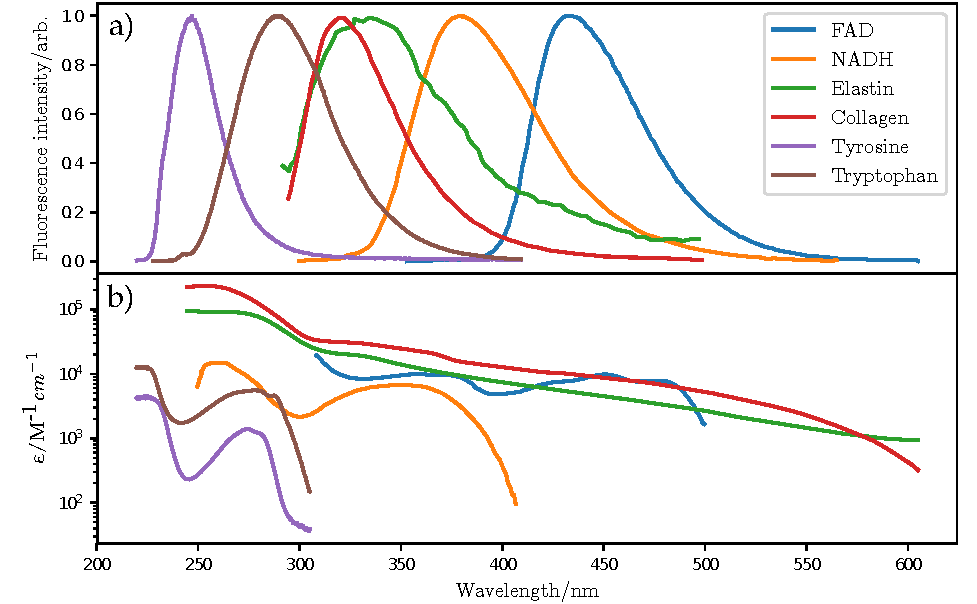
\includegraphics[width=.75\textwidth]{fluros.pdf}
  \caption{Top) Shows the fluorescent emission for the various different fluorophores. Bottom) Extinction coefficients for a selection fluorophores found in the skin~\cite{prahltyro,prahltryto,soltani2019deep,sun2012biomarkers,islam2013ph,evans2013magnetic,von2012fluorescence}.}
  \label{fig:flurosshow}
\end{figure}
% subsubsection optical_properties (end)
\FloatBarrier

\section{Modelling Fluorescence}

Fluorescence is the process in which light of a certain wavelength is incident on a molecule, the molecule absorbs the light and re-emits the light at a new longer wavelength.

\Cref{fig:Jabo} shows an example of Jablonski diagram.

\begin{figure}[!htpb]
	\centering
	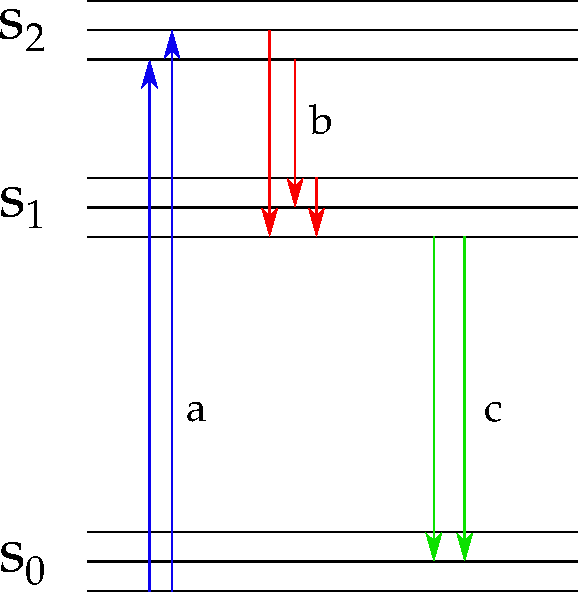
\includegraphics[width=0.45\textwidth]{jabo-diag.pdf}
	\caption{Jablonski diagram for PPIX. a) excitation of the ground state via absorption of a photon, b) non-radiative transition, and c) fluorescence.}
	\label{fig:Jabo}
\end{figure}

To model fluorescence from multiple fluorophores requires a change of the \gls*{mcrt} code presented thus far.
This change is to the interaction portion of the algorithm, so that it will now include the option for a packet to undergo fluorescence.
To calculate whether a packet absorbs, scatters or fluoresces, first the probability of each of these events must be calculated.
Discussion of scattering and absorption (by the bulk medium) was described in~\cref{sec:opticalprops}.
To calculate the probability of fluorescence, we first assume that the quantum yield of the molecule is unity.
This is physically unrealistic, however it does not affect the simulations accuracy, as modelling a realistic quantum yield would mean that more packets would be discarded, and thus the signal to noise ratio would be worse than if we assume a quantum yield of unity.
To calculate the probability of fluorescence, the absorption coefficient of the florescent molecule must be calculated.
This is shown in~\cref{eqn:flurodef}:

\begin{equation}
\mu_f=\ln\left(10\right)\varepsilon C
\label{eqn:flurodef}
\end{equation}

Where $C$ is the concentration of the fluorophore, $\varepsilon$ is the extinction coefficient of the fluorophore, and $ln(10)$ is the natural logarithm of 10\footnote{This factor appears as historically $\varepsilon$ was measured in base 10~\cite{jacques2013optical}.}.\\

The next step is to calculate the total attenuation coefficient for a given species as in~\cref{eqn:totdef}

\begin{equation}
\mu_{t_i}=\mu_{s_i}+\mu_{a_i}+\mu_{f_i}
\label{eqn:totdef}
\end{equation}

Where as usual $\mu_a$ and $\mu_s$ are the absorption and scattering coefficients, and $\mu_f$ is the fluorescence coefficient as defined in~\cref{eqn:flurodef}.
As the absorption coefficient of fluorophores are small in comparison to the medium, and that the absorption coefficient of fluorescent molecules are generally much larger than that of their scattering coefficient, we assume that the scattering coefficient is negligible.
Finally we calculate the probability of interacting with a given species using~\cref{eqn:totspec}

\begin{equation}
P_i=\frac{\mu_{t,i}}{\sum\limits_{i=1}^{N} \mu_{t,i}}
\label{eqn:totspec}
\end{equation}

Where $P_i$ is the probability of interacting with the $i^{th}$ species, the numerator is the attenuation coefficient for $i^{th}$ species, and the denominator is the total attenuation coefficient for all the species.

\cref{algo:speciespick} shows the process used to determine which species to interact with.

\begin{center}
\begin{algorithm}[H]
\SetAlgoLined
  set $\mu_{t_{i}}$\;
  set all $P_i$'s\;
  set $\xi_1$\;
  \uIf{$\xi_1 <= P_1$}{
    set $\xi_2$\;
    \uIf{$\xi_2 <= a_m$}{
      Scatter in medium\;
     }
     \Else{
      Absorb in medium\;
     }
  }
  \uElseIf{$\xi_1 <= P_1 + P_2$}{
    Species 1 fluoresces\;
  }
  \uElseIf{$\xi_1 <= P_1 + P_2 + P_3$}{
    Species 2 fluoresces\;
  }
  \uElseIf{$\xi_1 <= P_1 + P_2 + P_3 + ... + P_n$}{
    Species n fluoresces\;
  }
  \Else{
    Error, no interaction\;
  }
\
\caption{\textit{An algorithm to determine which species to interact with. $P_1$ is the probability of interacting with the bulk medium, $P_2$ to $P_n$ is the probability of interacting with a fluorescent species, $a_m$ is the albedo of the bulk medium, $\xi_i$ is a random number, and $\mu_{tot}$ is the total attenuation coefficient of all the species summed.}}
\label{algo:speciespick}
\end{algorithm}
\end{center}

This method allows an arbitrary number of fluorophores to be modelled.
To ensure that this method works as intended, the method is compared to experimental data taken by Campbell \textit{et al.}~\cite{louisethesis}.

The cuvette was filled with Intrlipid $20\%$ diluted with water, and a fluorescent agent Coproporphyrin III\@.
The total volume of this mixture was $6~ml$, consisting of $1~ml$ of Coproporphyrin III, $4.99~ml$ of water, and $0.0~1ml$ of Intrlipid $20\%$, of which $2~ml$ was pipetted into the cuvette.
$405~nm$ light was shone on a cuvette of area $10~mm \times 10~mm$., and collected via the same fiber, of diameter $600~\mu m$.
The fiber has a NA of 0.22.
The signal is the recorded by a blah blah blah..

\begin{figure}[!htpb]
	\centering
	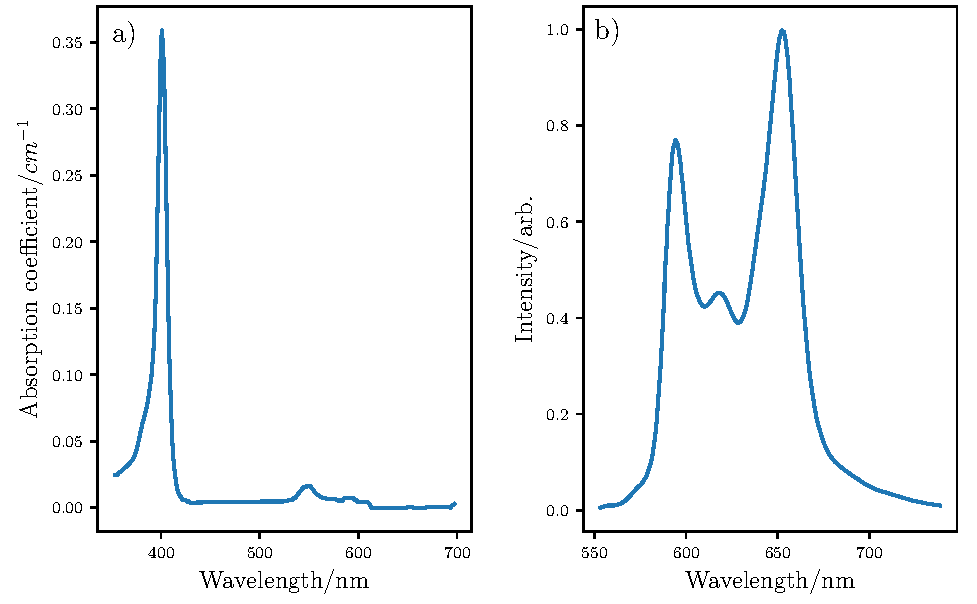
\includegraphics[width=0.75\textwidth]{cop-optprop.pdf}
	\caption{Optical properties of Coproporphyrin III. The figure on the left shows the absorption coefficient as a function of wavelength. The figure on the right shows the emission spectrum as a function of wavelength.}
	\label{fig:coporiii}
\end{figure}

The simulation is setup to mimic the experimental setup.
A medium of $10~mm^3$ is used with 1 voxel to increase the speed of computation.
As before Intralipid is assumed to be wholly scattering with no absorption, so an albedo of 1 is used.
Conversely the Coproporphyrin III is wholly absorbing with no scattering.
Coproporphyrin III absorption spectrum is as shown along side its emission spectrum in~\cref{fig:coporiii}.
If a photon packet leaves the top face of the simulated medium, within the radius of the fiber at an angle the fiber could accept, then the packet is recorded.
The simulation is run with $10^7$ photons which yielded~\cref{fig:flurovalid}.

\begin{figure}[!htpb]
  \centering
  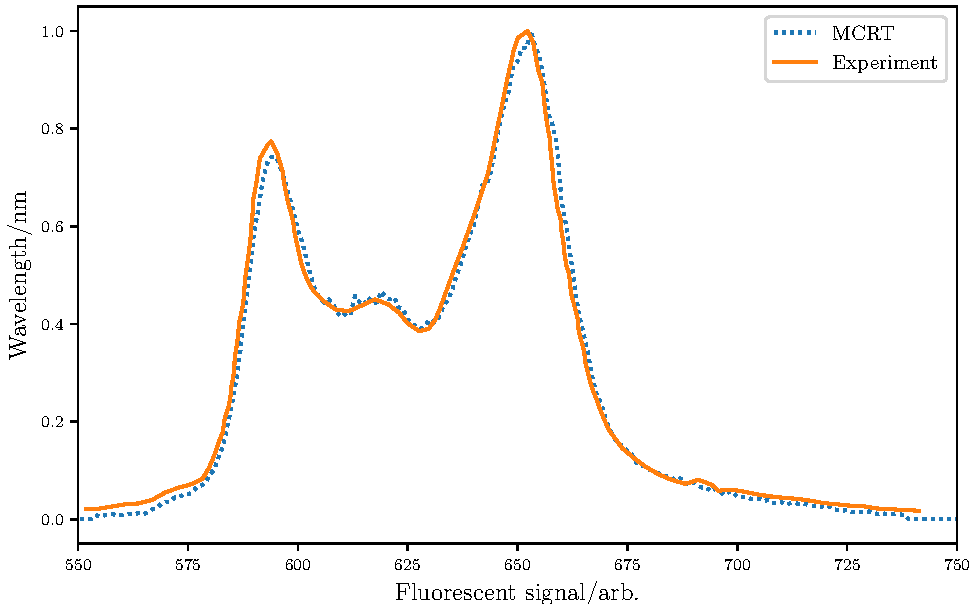
\includegraphics[width=0.75\textwidth]{Fluro-valid.pdf}
  \caption{Validation of florescence modelling technique as described above. Figure shows that the MCRT method matches closely to the experimental results.}
  \label{fig:flurovalid}
\end{figure}

\FloatBarrier

\section{Nelder-Mead Method}

The \gls*{nm} method is an algorithm for unconstrained optimisation. 
The algorithm is based upon iteratively updating a simplex. 
A simplex is a structure in $n dimensional$ space, consisting of $n+1$ points that are not in the same plane. 
Therefore in 1D, the simplex is a line, in 2D a triangle, in 3D a tetrahedron, etc. 
The Nelder-Mead method is a gradient free method, meaning that it does not require derivatives to be calculated and that the search space does not need to be smooth.
This makes it ideal for problems where derivates are not able to be computed easily, or the search space is not smooth.
However, the NM method can also get stuck at local minima so care must be taken to avoid this.

The NM algorithm works by removing the worst vertex of the simplex and replacing it with a ``better'' vertex calculated via a number of different operations.
These operations can be seen in~\cref{fig:NM-operations}.\\

The first step of the~\gls*{nm} method is to sort the initial vertices according to their fitness.
For $n=2$, we define $x_w$ as the ``worst'' point, $x_l$ and the ``lousy'' point, and $x_b$ the ``best'' point, such that $f(x_b)\leq f(x_l)\leq f(x_w)$, where $f(x)$ is evaluating the `fitness' of a point $x$. 
The fitness function varies from problem to problem, and usually takes the form of the function that is being optimised.

With the vertices sorted, the centroid of the simplex is calculated as in~\cref{eqn:centroid}.
The centroid is the mean of all the vertices bar the ``worst'' point.

\begin{figure}[!htbp]
    \centering
    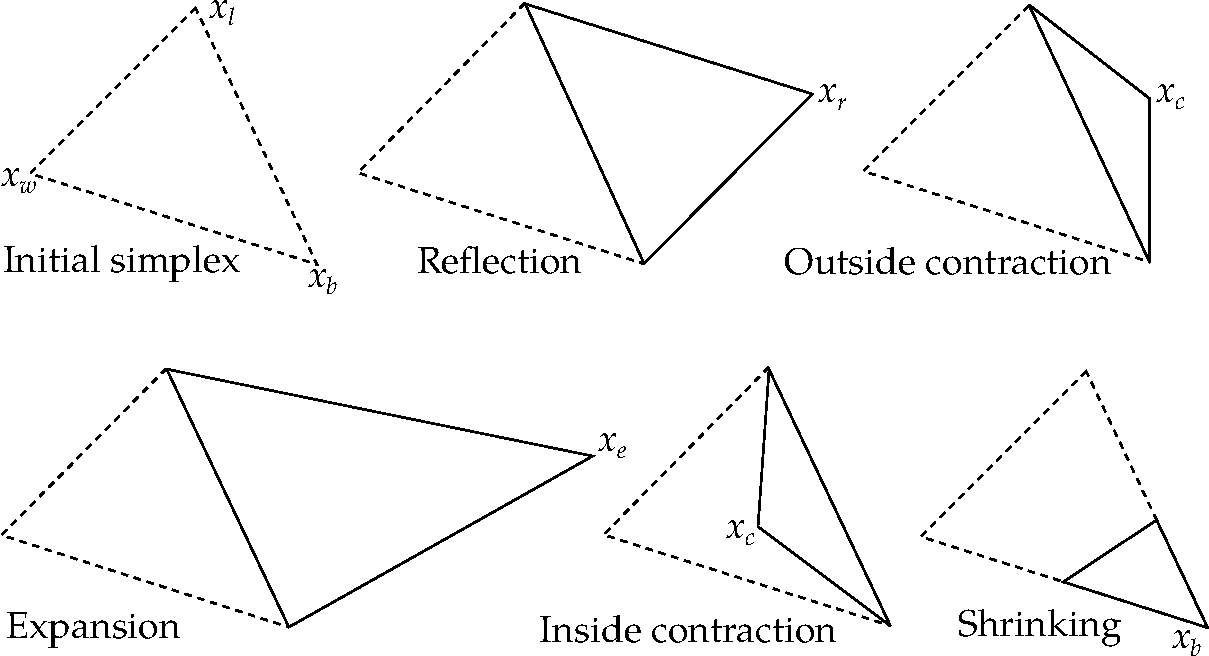
\includegraphics[width=0.75\textwidth]{simplex-operations.pdf}
    \caption{Operations that can be preformed on a simplex for $n=2$.}
    \label{fig:NM-operations}
\end{figure}

The next step is to move the simplex via a reflection.
To calculate the new vertex via reflection~\cref{eqn:reflect} is used, where $\alpha$ is the reflection factor.
If this new point, $x_r$, is better\footnote{Here better means the point has a lower fitness score} than the current ``best'' point then we calculate a new point in the same direction but further using the expansion operation~\cref{eqn:expand}, where $\gamma$ is the expansion factor.
If this new point, $x_e$, is better than the ``best'' point then we replace $x_w$ with $x_e$ and start the process again.
However, is $x_e$ is not better than the ``best'' point, then we discard it and replace the worst point with $x_r$ the reflected point.

If when calculating $x_r$, we find that is worse than the ``best'' point, we then check if $x_r$ is better than the `lousy' point.
If $x_r$ is better than $x_l$ then we replace the ``worst'' point and start the process again.
However, if the $x_r$ is worse than $x_l$, we then compare it to the ``worst'' point.
If $x_r$ is better than the ``worst'' point then we preform and inside contraction~\cref{eqn:insidecontract}, where $\beta$ is the contraction factor.
If this new point, $x_{ic}$, is better than the ``worst'' point then we keep it, otherwise we preform the shrink operation, shrinking the whole simplex around the ``best'' point.

If $x_r$ is not worse than the ``worst'' point then we preform an outside contraction~\cref{eqn:outsidecontract}.
This computes a new point $x_{oc}$.
If $x_{oc}$ is better than $x_w$, then we keep it, otherwise again we shrink around the ``best'' point.
The process described above is summarised in~\cref{fig:NM-algo}.

Standard values for the factors are: $\alpha=1$, $\beta=\frac{1}{2}$, and $\gamma=2$.
Though in practice these values are adjusted for the problem at hand.
For higher dimensions, i.e. where $n > 2$ F. Gao \textit{et al}. suggest that the parameters should be changed based upon how many dimensions are used for the simplex~\cite{gao2012implementing}.
The values F. Gao \textit{et al} suggest are: $\alpha=1$, $\beta=1+\tfrac{2}{n}$, $\gamma=0.75-\tfrac{1}{2n}$, and $\delta=1-\tfrac{1}{n}$.
Where $n$ is the order of dimensions.

\begin{align}
c &= \frac{1}{n}\sum \limits_{i=1,i\neq w}^{n+1} x_i \label{eqn:centroid}\\
x_r &= c + \alpha(c - x_w)\label{eqn:reflect}\\
x_e &= c + \gamma(x_r - c)\label{eqn:expand}\\
x_{oc} &= c + \beta(x_r - c)\label{eqn:outsidecontract}\\
x_{ic} &= c + \beta(x_w - c)\label{eqn:insidecontract}
\end{align}

As the Nelder-Mead method has no inbuilt convergence criteria, this must be added.
We use two different criteria based upon simplex size, and vertex fitness.
The criteria for the simplex size is as; The size of the simplex is calculated using~\cref{eqn:sizeof}:

\begin{equation}
size=\sum\limits_{i=1}^{n+1}|p_{i}-p_{i+1}|
\label{eqn:sizeof}
\end{equation}

Where $p_i$ and $p_{i+1}$ are vertices in the simplex that are connected by an edge. 
If the size of the simplex falls below a pre-set value, then we preform a factorial test to see if the simplex should be restarted or if the algorithm should terminate.
The factorial test checks the space around the current simplex to ensure that we have converged to a global minima.
If the check fails then the algorithm is restarted with the current best point kept, and new vertices generated.

\begin{figure}[!htbp]
    \centering
    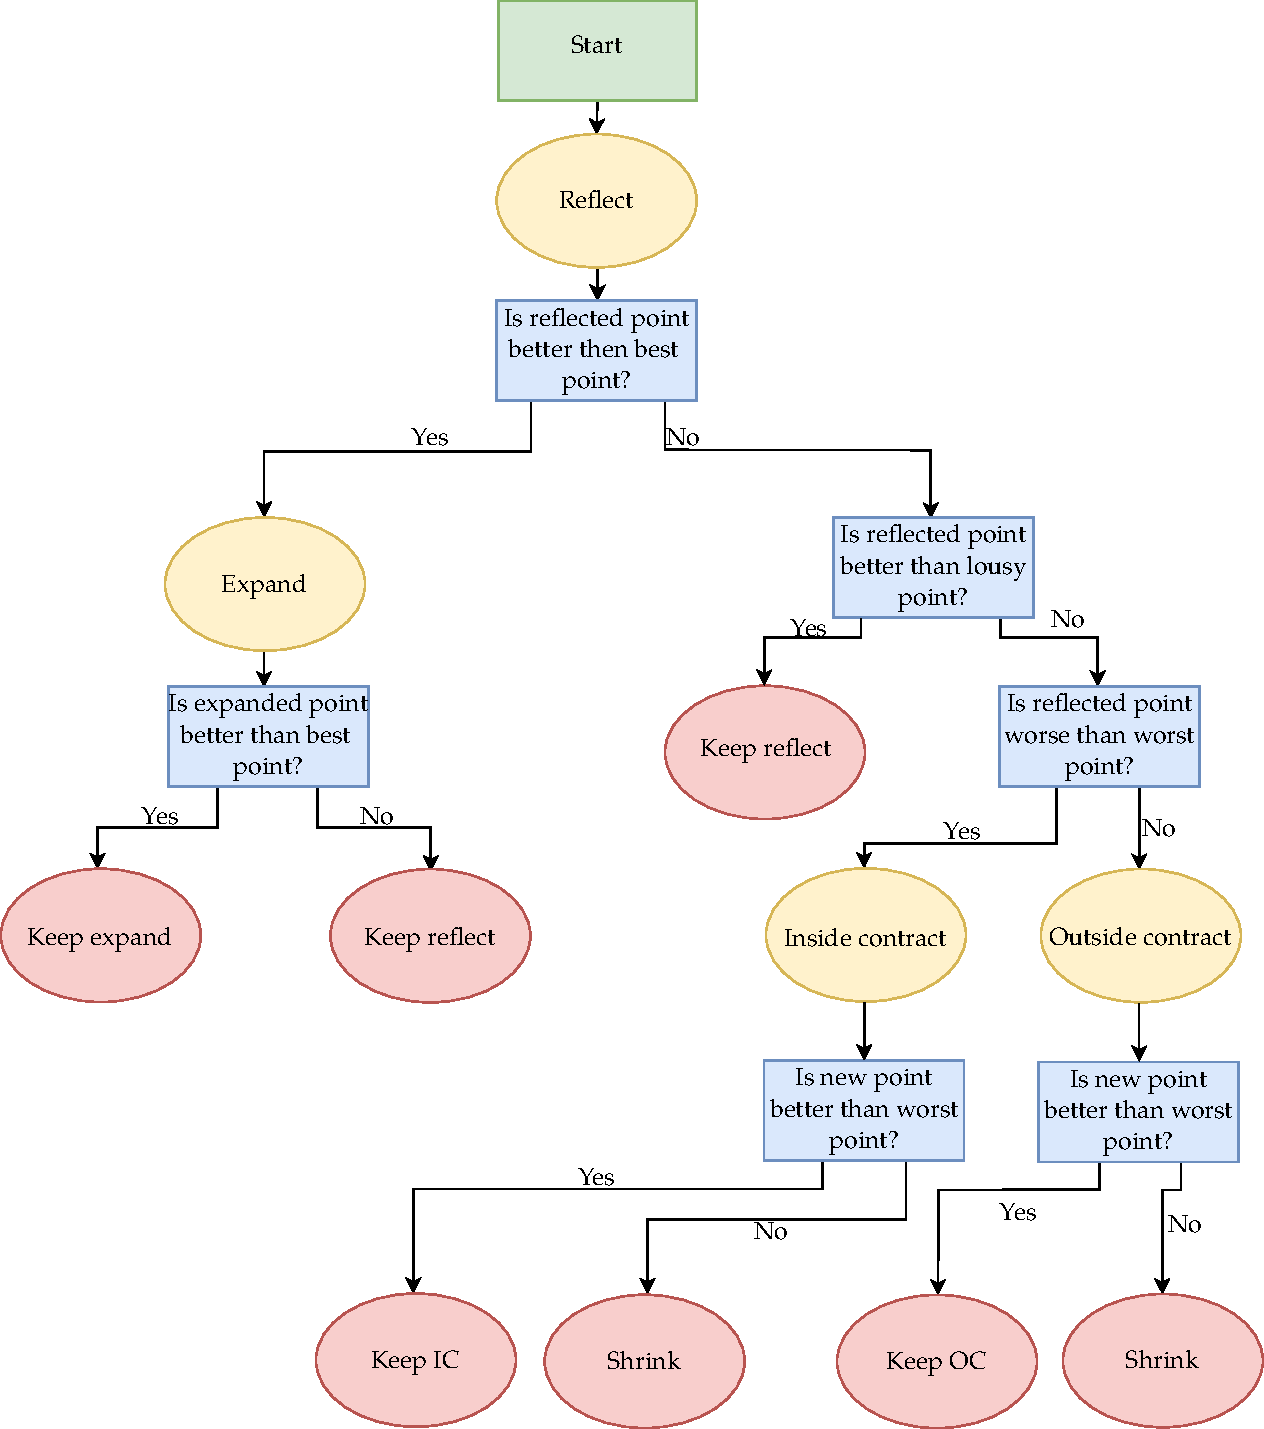
\includegraphics[width=0.65\textwidth]{flowchart-nelder.pdf}
    \caption{Nelder-Mead decision tree.}
    \label{fig:NM-algo}
\end{figure}

The other convergence criteria is a check to see if the best point is ``good enough''.
The current best point is compared to a pre-set fitness value.
If the best point is better than the pre-set value then the algorithm terminates.

\FloatBarrier
\section{Validation}
The~\gls*{nm} method was coded in modern Fortran, so that it could be easily interfaced with the~\gls*{mcrt} code developed as part of this thesis.
To test that the \gls*{nm} method works as intended a number of trial optimisation functions were tested, see~\cref{tab:testfuncs}.
This was achieved by selecting an initial simplex, and the method allowed to iterate until it converged.
The results of this are shown in~\cref{fig:nmtest}.


\begin{table}[!htbp]
    \begin{tabular}{|c|c|c|}
    \hline
        Name         & Formula                                                                & Global Minumum                \\ \hline
        Sphere       & $x^2+y^2$                                                              & $f(0,0)=0.$                   \\ \hline
        Rosenbrock   & $(a-x)^2+b(y-x^2)^2$                                                   & $f(1,1)=0.$                   \\ \hline
        Ackely       & $ -20\exp\left[-0.2\sqrt{0.5\left(x^{2}+y^{2}\right)}\right] - $       & $f(0,0)=0.$                   \\
                     & $\exp\left[0.5\left(\cos 2\pi x + \cos 2\pi y \right)\right] + e + 20$ &                               \\ \hline
        Himmelblau's & $(x^2+y-11)^2+(x+y^2-7)^2$                                             & $f(3,2)=0., $                 \\
                     &                                                                        & $f(-2.805118,3.131312)=0.,$   \\
                     &                                                                        & $f(-3.779310,-3.283186)=0.,$  \\  
                     &                                                                        & $f(3.584428,-1.848126)=0.$    \\ \hline
    \end{tabular}
    \caption{Table of standard test functions for numerical optimisation.}
    \label{tab:testfuncs}
\end{table}


\begin{figure}[!htbp]
    \centering
    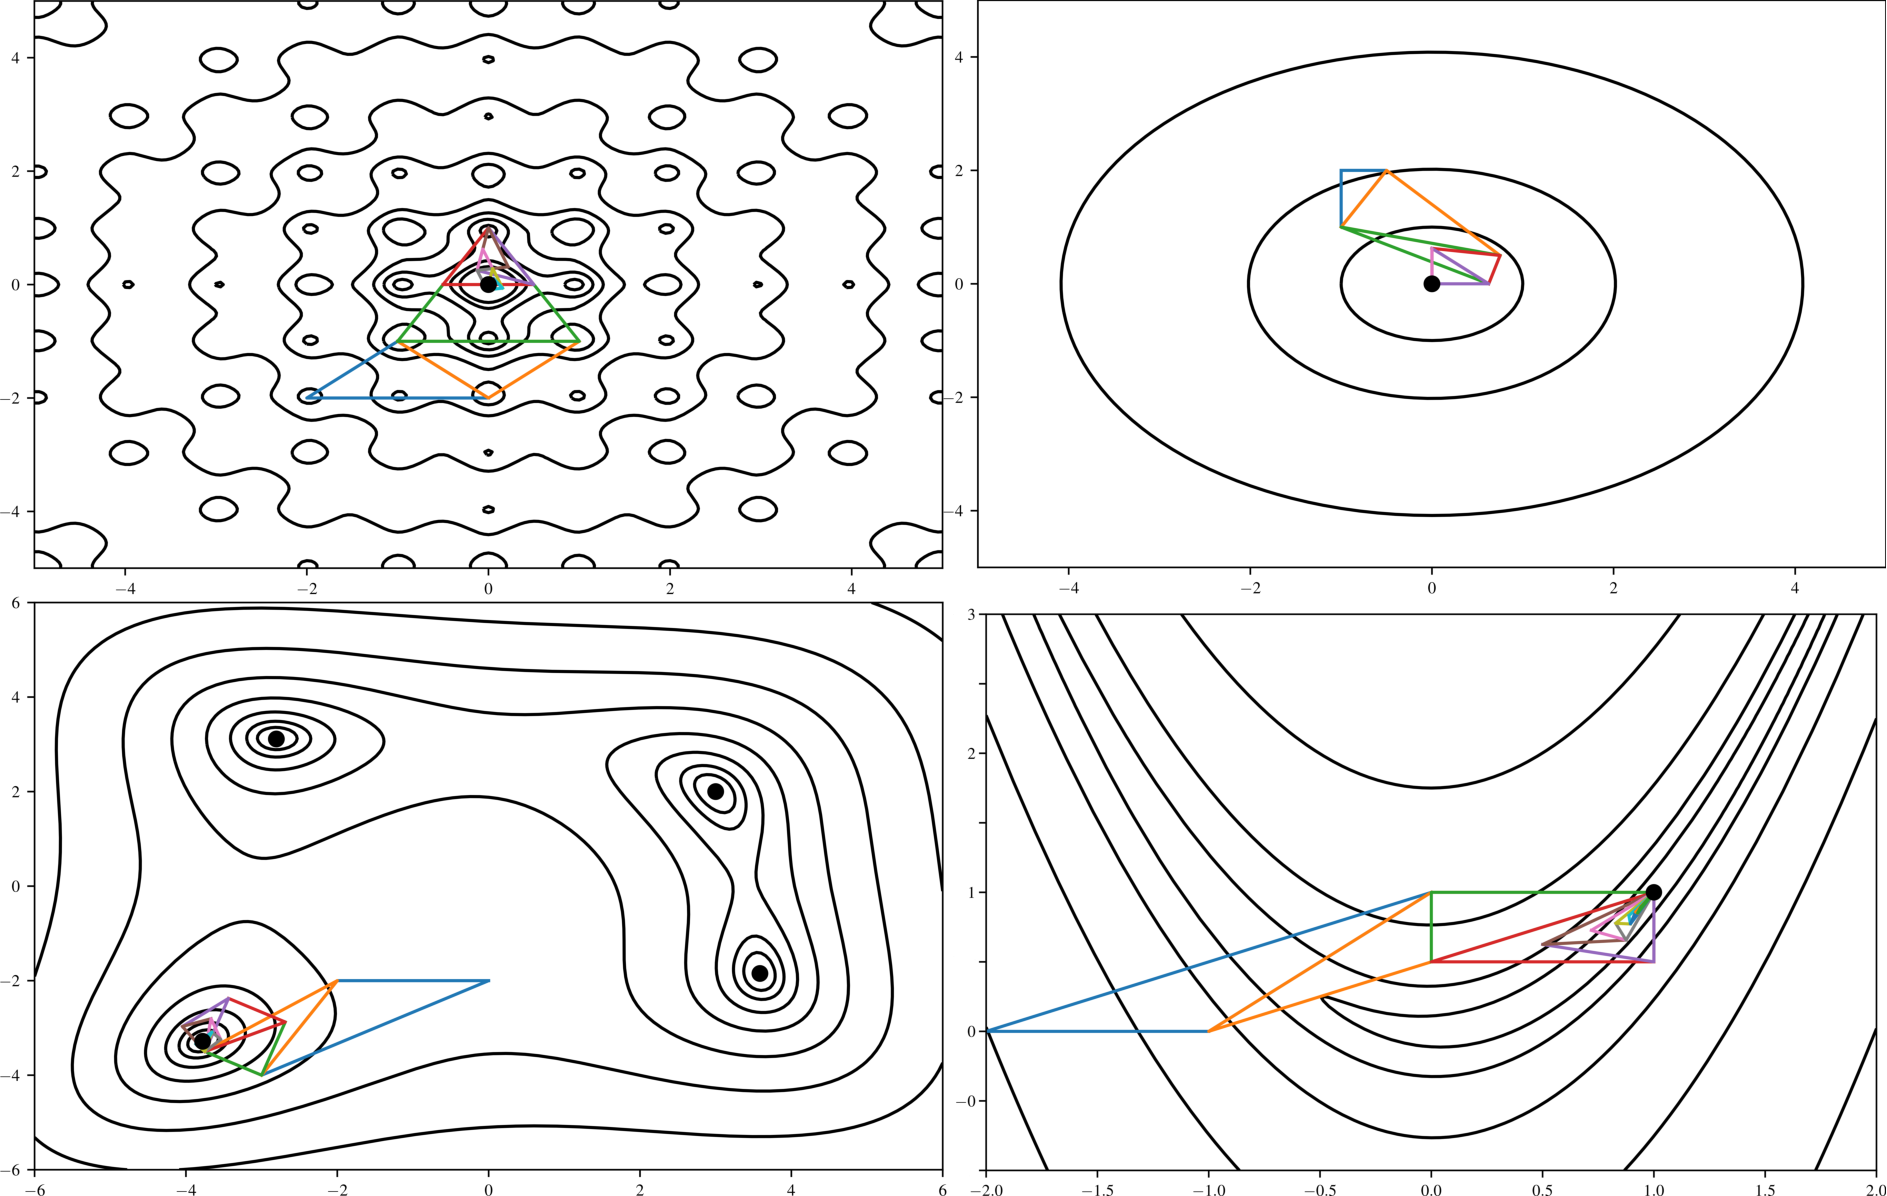
\includegraphics[width=0.75\textwidth]{all-nm-tests.pdf}
    \caption{Contour plots of test functions with Nelder-Mead simplexes over plotted. Top left is the Ackely function, top right is the sphere function, bottom left is the Himmelblau's function, and the bottom right is the Rosenbrock function. Blue simplex is the initial simplex, and the large black dots represent the Global minima.}
    \label{fig:nmtest}
\end{figure}

Some of these functions (Sphere, and Rosenbrock's) can also be extended to arbitrary dimensions. These functions were used to check that the NM method works as intended in these higher dimensions where the NM method will primarily be used in this thesis.

To ensure that the~\gls*{nm} method can be used to find the unknown concentrations of the autoflurophores, we test the method with a two different toy models.
The first model is a 2D model,with two different fluorophores evenly distributed over all 5 layers of our skin model. 
This two different fluorophores are NADH, and a fictitious fluorophore that has similar properties to FAD and tryptophan, such that the excitation spectrum is that of NADH and the emission spectrum is that of tryptophan.
The concentration in these layers is such that the bulk optical properties are not affected: NADH has a concentration of $1.0~\mu M$, and the fictitious fluorophore has a concentration of $2.5~\mu M$.
To generate a spectrum to which the \gls*{nm} method can compare to, the \gls*{mcrt} code is run with the above configuration of fluorophores.
This generated~\cref{fig:toymodelspectra}.


\begin{figure}[!htbp]
  \centering
  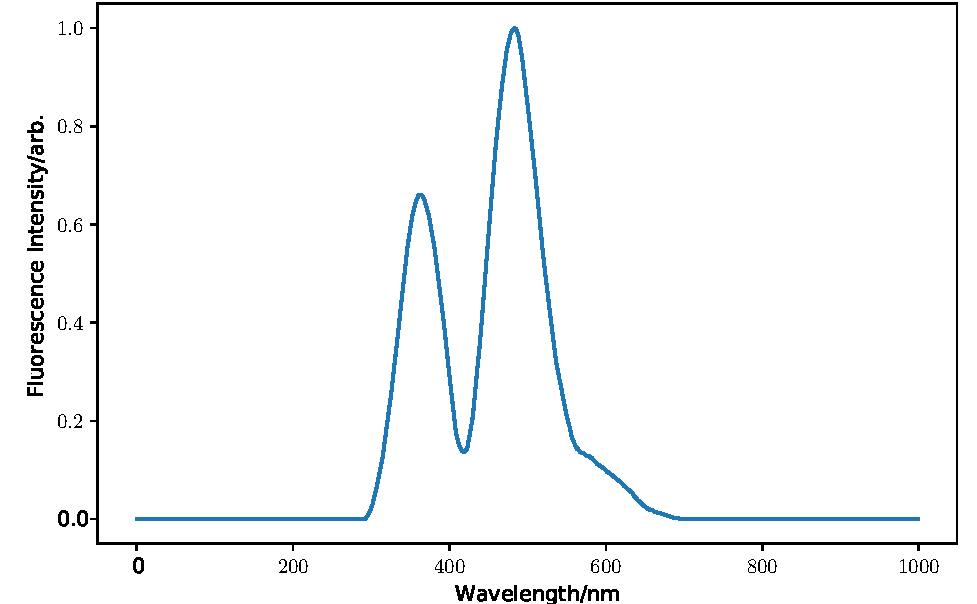
\includegraphics[width=0.6\textwidth]{target-toy.pdf}
  \caption{Example of toy model spectrum for testing NM method. The two peaks correspond to the fictitious fluorophore, and NADH.}
  \label{fig:toymodelspectra}
\end{figure}

The fitness function chosen to check whether the NM method is converging to the generated spectrum is as:

\begin{equation}
fitness = \sum\limits_{i=1}^{n}(x_i-m_i)^2
\end{equation}

Where $x_i$ is a data point at a wavelength $\lambda_i$ produced by the MCRT, and $m_i$ is a data point in the model at a wavelength $\lambda_i$.

As the \gls*{nm} can get stuck in local minima, we run the method for several different initial simplices to ensure that the method does not get stuck in a local minima.
As many calls to the \gls*{mcrt} code need to be done, and the fluorophore concentration is low this means that many packets need to be run to achieve a good single to noise ratio.
These two conditions result in a computational load that is infeasible to run. 
Therefore the~\gls*{mcrt} algorithm has to be computationally efficient in order to arrive at an answer within a reasonable time.
To this end the 3D skin model is shrunk to a 1D model in the z direction so that the optical integration routine can efficiently move the packet through the simulated medium.
The optical properties of the incident wavelength are also stored so that when a new packet is started the optical properties can easily be adjusted without need for any calculation.
Finally a filter is employed on the output fluorescence spectrum to smooth the noise out.
The filter used is a Savitzky-Golay filter.
This filter fits multiple low-degree polynomials to subsets of the data, thus smoothing the data~\cite{press1990savitzky}. 
\Cref{fig:sgfilter} shows the use of the Savitzky-Golay filter on sample output data from the \gls*{mcrt} simulation.

\begin{figure}[!htbp]
  \centering
  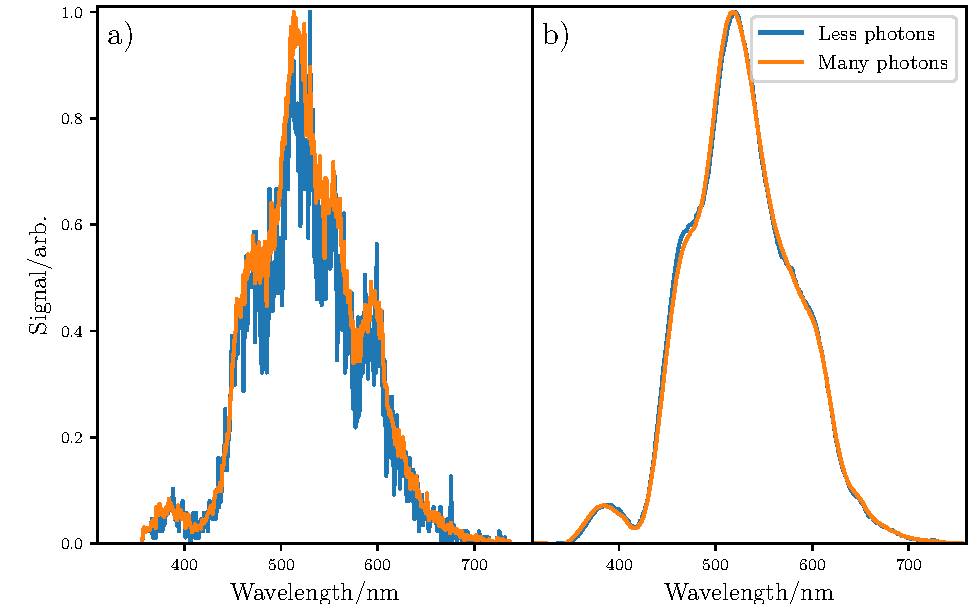
\includegraphics[width=0.75\textwidth]{sgfilter-prrof.pdf}
  \caption{Illustration of how the Savitzky-Golay filter works on noisy data and recovers the roughly the same signal on the same dataset with less noise. Left image shows the raw signal for a simulation run with less photons and more photons. Right image shows the dataset after the Savitzky-Golay filter is applied.}
  \label{fig:sgfilter}
\end{figure}


Using the above set-up with the Savitzky-Golay filter on the output spectrum, allowed the \gls*{nm} method to efficiently run many model of various different concentrations and ``find'' a set of concentration that resulted in a close match with the target spectrum.
However, as the detected fluorescence spectra are normalised to their peak values we cannot use this method to determine the original concentration, but rather the ratio between the two concentration.
\Cref{fig:spaceplot2D} shows the search space and the spread of the concentration values calculated by the \gls{nm} method compared to the original target concentration.
The spread of the concentrations calculated by the \gls*{nm} method follow a linear relationship as would be expected.
Therefore a line of best fit was fitted to the concentrations.
This yielded a line ($y=m\ x$) with $m=2.49\pm0.05$.
The expected relation between the concentration is where $m =2.5$ therefore, the \gls{nm} method can be used to determine the relative difference in concentrations within one standard deviation.


\begin{figure}[!htpb]
  \centering
  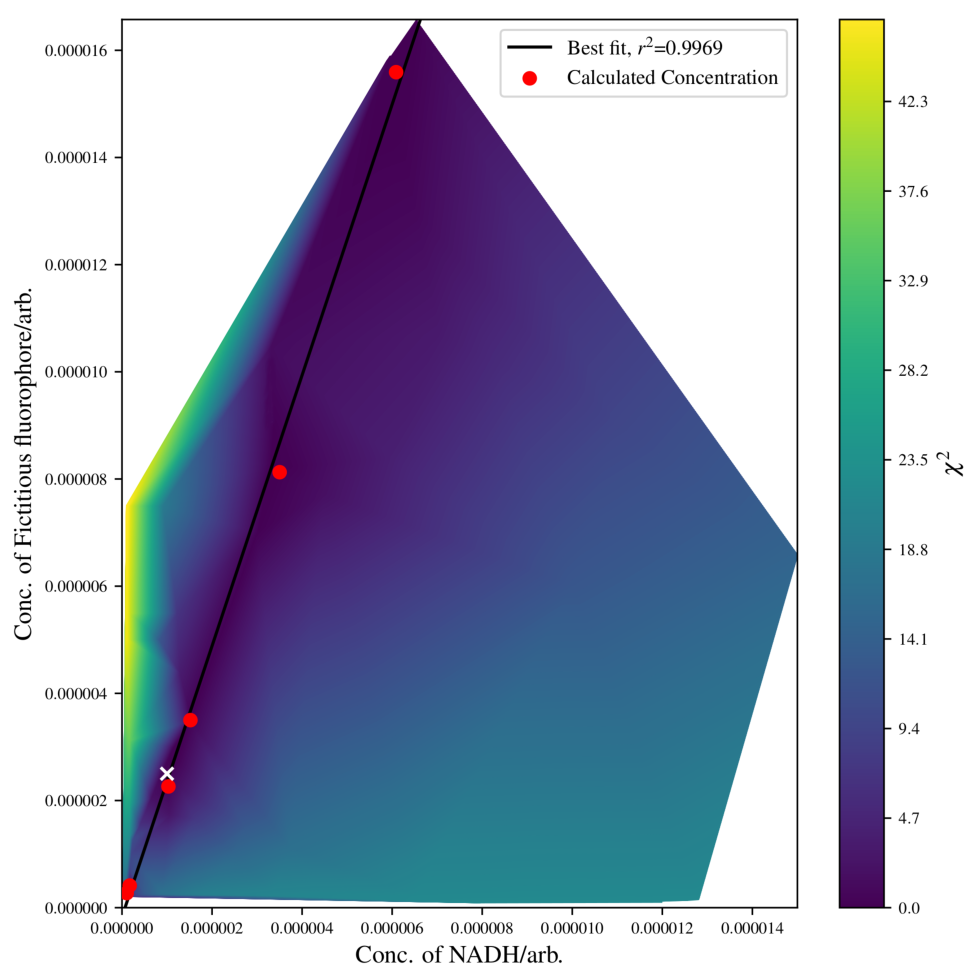
\includegraphics[width=0.75\textwidth]{2d-space-plot-thesis.pdf}
  \caption{Figure shows the search space for the 2D toy problem outlined above. A line of best fit is fitted to the concentrations found by the \gls*{nm} method. Note also the valley of good fit where the line of best fit lies. The search space is also fairly smooth.}
  \label{fig:spaceplot2D}
\end{figure}


The \gls*{nm} method was also tested on a toy model for $n=3$.
Here the fluorophores used were: NADH, FAD, and a fictitious fluorophore with the absorption properties of NADH and the emission properties of Tyrosine.
The fluorophores had concentrations of $1.05\mu M$ $525\mu M$, and $125\mu M$ respectively.
The set-up is the same for the above $n=2$ case, with the same filter and computational speed ups used.
\Cref{fig:3dtoymodel} shows various concentrations as calculated by the \gls*{nm} method compared to the original concentration.
Again a line of best fit was fitted to the calculated points.

\begin{figure}[!htpb]
  \centering
  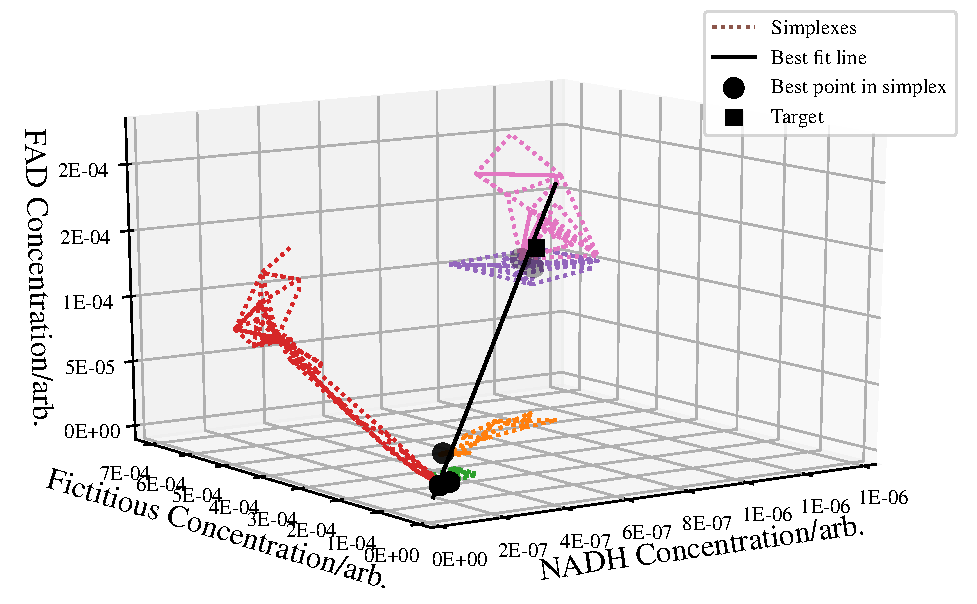
\includegraphics[width=0.75\textwidth]{3d-nm-example.pdf}
  \caption{Figure shows the line of best fit for the case where $n=3$. Figure also shows the simplices path over their whole lifetime, from initial guess to final simplex.}
  \label{fig:3dtoymodel}
\end{figure}


\begin{figure}[!htpb]
  \centering
  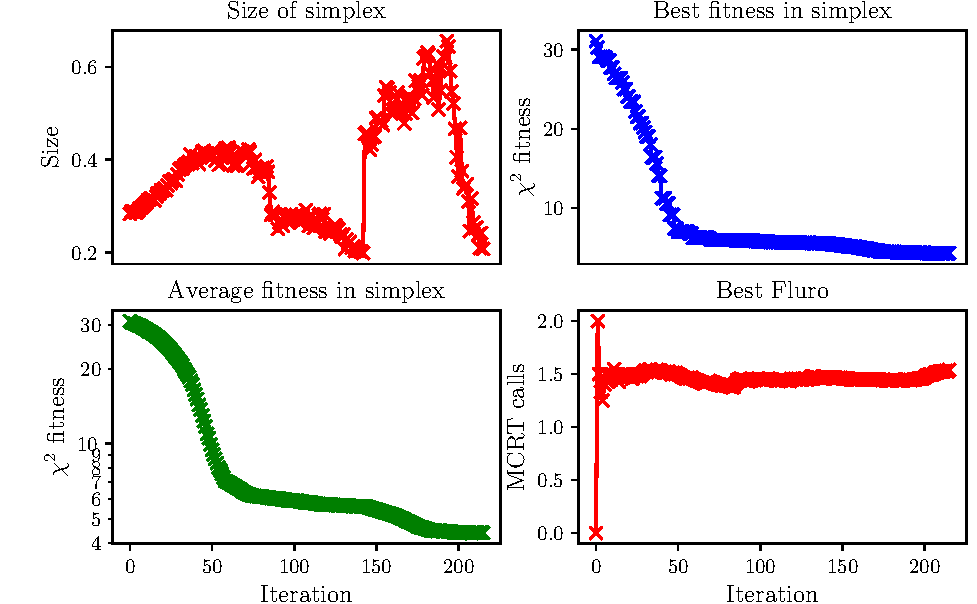
\includegraphics[width=0.75\textwidth]{NM-update.pdf}
  \caption{blah}
  \label{fig:NMupdate}
\end{figure}




\FloatBarrier
\section{Results}

Before running the NM method on the experimental data, the fluence of the input and fluorescence light is analysed alongside the location as a function of depth of the fluorescent light.

\Cref{fig:uvpen} show the fluence as a function of depth for the incident UV light.
The figure shows that most of the incident light is contained within the top three layers, with little getting to the Reticular dermis, with none reaching the Hypodermis.

\Cref{fig:fadnadhboth} shows the fluence of detected fluorescent light (see~\cref{app:lightdect} for discussion of how this is tracked.).
The figure shows that the fluence is highest in the Papillary dermis this is due to a number of reasons.
First the refractive indices of the layers are different, this can lead to light getting ``trapped'' in a layer as it maybe reflected of the layer boundary.
Second, fluorescent light is emitted isotropically which means that fluorescent light emitted in the upper layers of the skin, may be emitted in the direction of the Papillary dermis.
Finally the optical properties also have an effect on the detected light fluence.
***expand on this more once I have plotted the optical properties ***

\begin{figure}[!htpb]
    \centering
    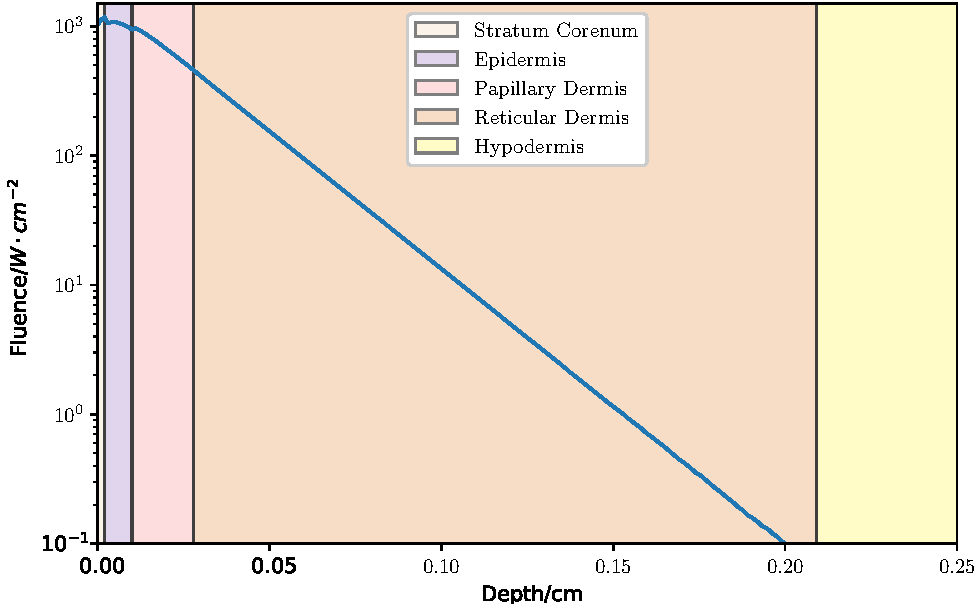
\includegraphics[width=0.75\textwidth]{UV-fluence-365nm.pdf}
    \caption{Penetration of UV radiation as a function of depth.}
    \label{fig:uvpen}
\end{figure}

\begin{figure}[!htpb]
    \centering
    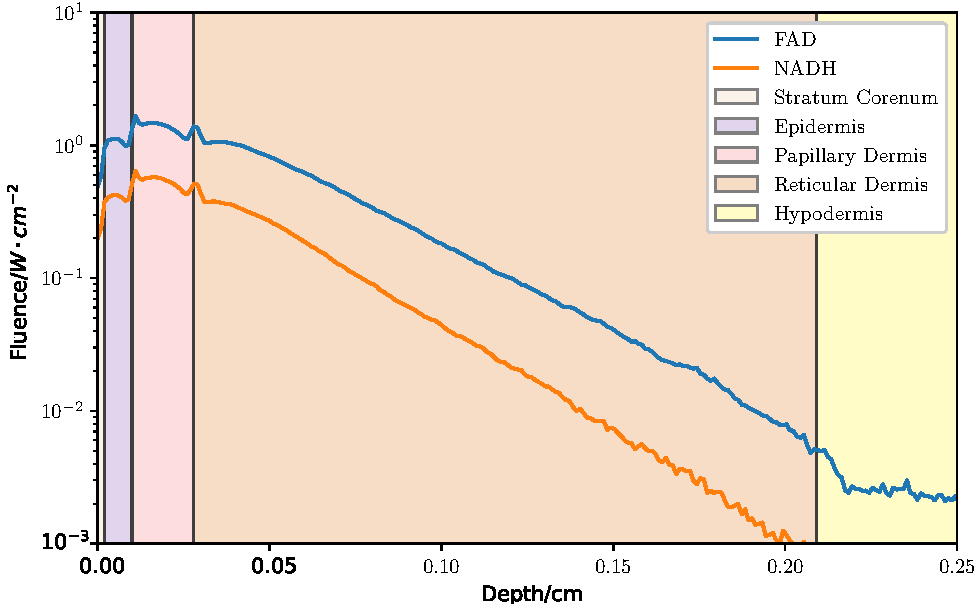
\includegraphics[width=0.75\textwidth]{FAD.pdf}
    \caption{Detected fluence for FAD and NADH fluorescence.}
    \label{fig:fadnadhboth}
\end{figure}

\begin{figure}[!htpb]
    \centering
    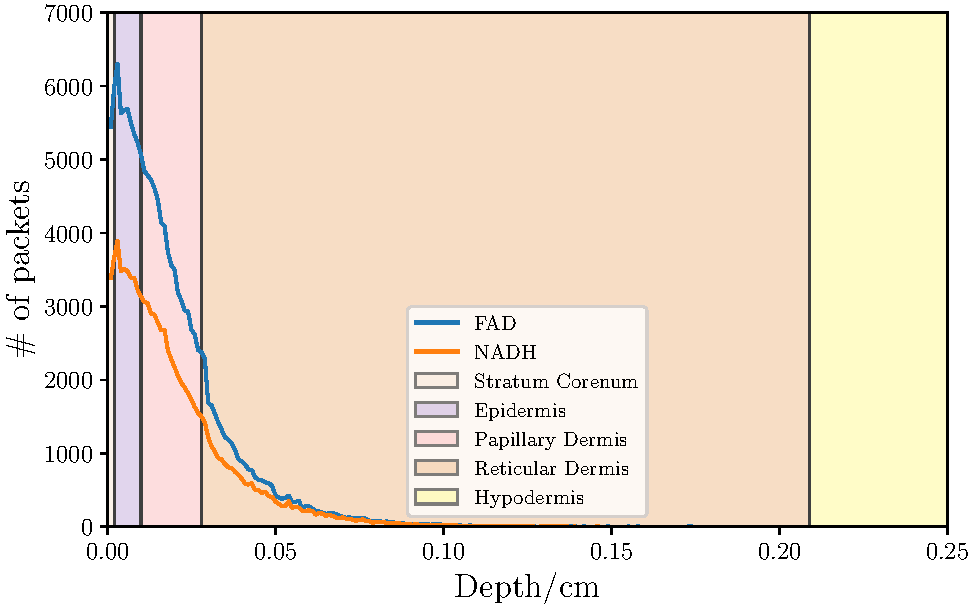
\includegraphics[width=0.75\textwidth]{fluro-loc.pdf}
    \caption{Amount of packets escaping as a function of depth for FAD and NADH fluorescence.}
    \label{fig:floc}
\end{figure}

\begin{figure}[!htpb]
    \centering
    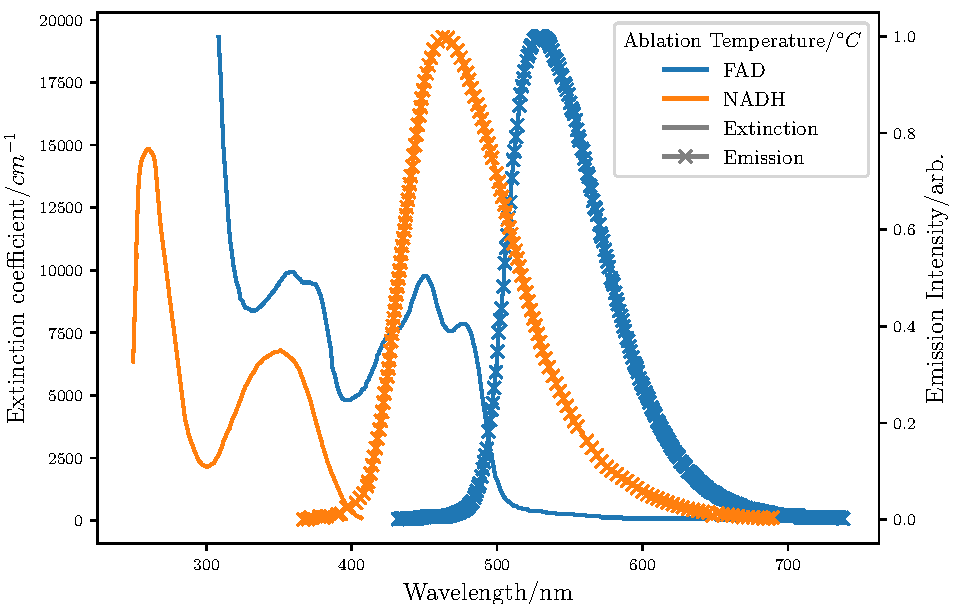
\includegraphics[width=0.75\textwidth]{show-eps-and-fluro-out.pdf}
    \caption{NADH and FAD absorption and emission spectra.}
    \label{fig:epsfluro}
\end{figure}

\begin{figure}[!htpb]
    \centering
    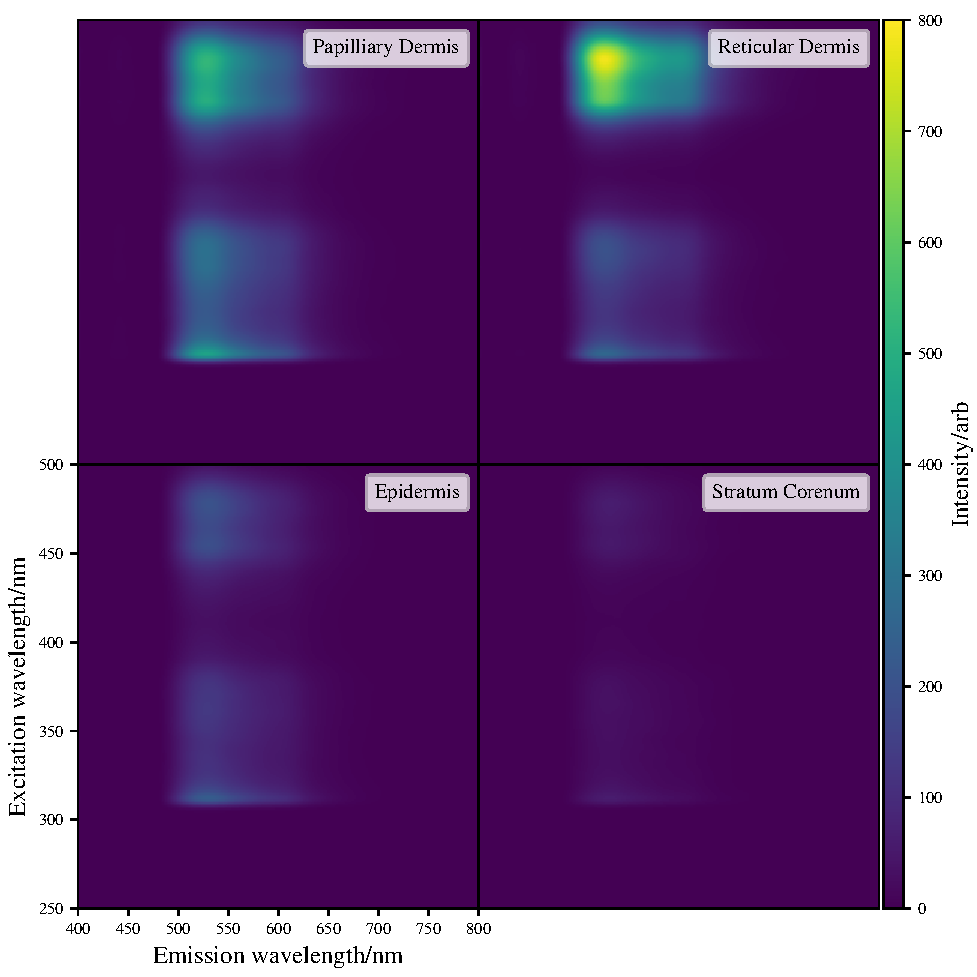
\includegraphics[width=0.75\textwidth]{FAD-eem.pdf}
    \caption{eem-esque map of FAD fluro.}
    \label{fig:fadeem}
\end{figure}

\begin{figure}[!htpb]
    \centering
    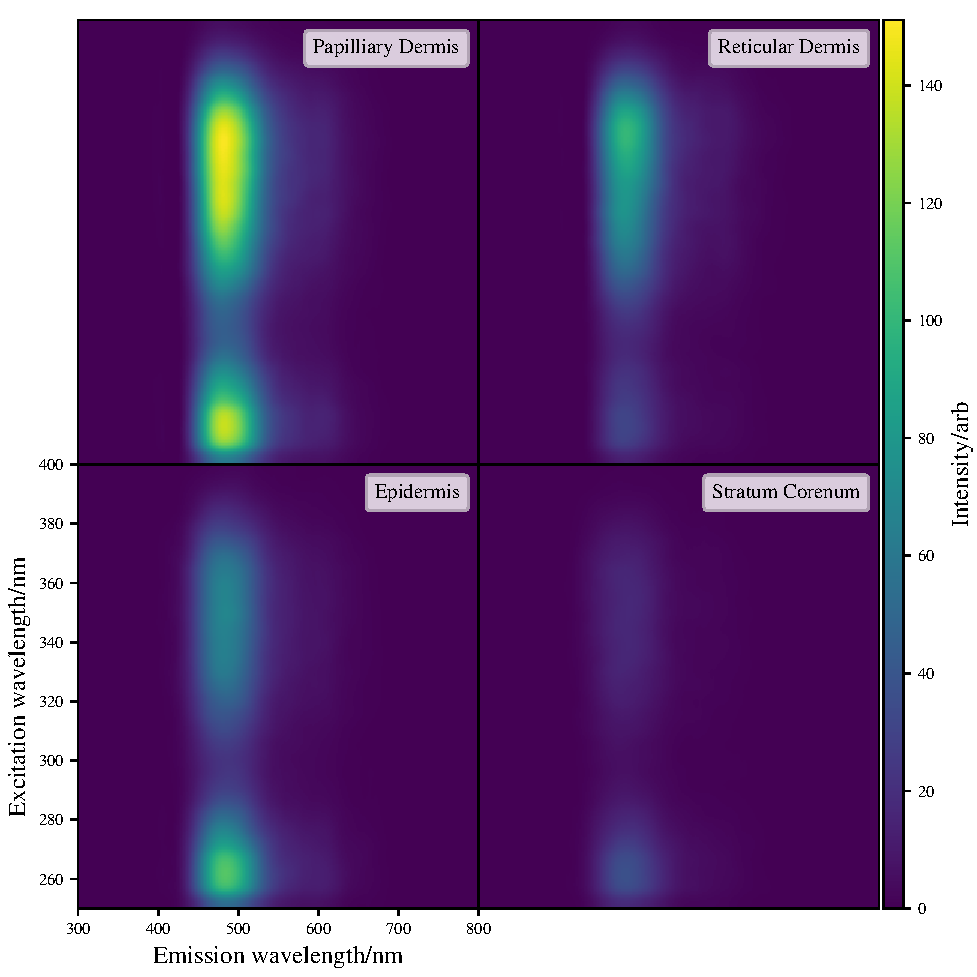
\includegraphics[width=0.75\textwidth]{NADH-eem.pdf}
    \caption{eem-esque map of NADH fluro.}
    \label{fig:nadheem}
\end{figure}

\section{Discussion}

\section{Effect of Tissue Optics on Fluorescent Signal}

One of the problems in using autofluroescence as a biomarker for various diseases is that information about which fluorophore you are measuring can be hard blah blah

use eem

fad from diff layers
nadh from different layers


\section{Future Work}

\section{Conclusion}

We have presented out code, AmoebaMCRT, which combines the Nelder-Mead method and MCRT in order to determine the concentrations of naturally occurring fluorophores in human skin.


%AF Code works, tested against toy model, may need further validation. 

%No paper or aim for project. Need contact with Dundee/Ninewells to proceed.
